\chapter{EXPERIMENT 2: AN INVESTIGATION OF SHALLOW PROCESSING} \label{ch:exp2}

The previous chapter focused on the role of local ambiguity in agreement attraction and investigated an alternative explanation for existing Turkish agreement attraction effects: reduced subjecthood association. Our results showed that the local ambiguity on the head noun does not seem to affect either the presence or the magnitude of the grammaticality illusion.

This chapter aims to investigate yet another explanation for existing Turkish agreement attraction effects: form-driven processing strategy. In the light of recent findings in psychology and psycholinguistics, one can stipulate that participants do not comprehend all details of lexical, semantic, or discourse-related information \citep{ChristiansonEtAl2001}. Instead, they may have a rough understanding of the sentence or use specific strategies to answer questions while having a limited understanding of the sentence. This chapter investigate whether participants both in our experiment and \cites{LagoEtAl2015} experiment were using additional strategies that relies on the phonological form. We present two experiments in which we abuse the homophony between the nominal and the verbal plural marking in Turkish. 

\section{Shallow processing in agreement attraction}

Having discussed an alternative hypothesis based on local ambiguity and reduced subjecthood association, we focus on another alternative theory that stems from Turkish' unique feature. Unlike other languages that exhibited agreement attraction effects, the Turkish verbal agreement marker and nominal plural marker share the same form: \emph{-lAr}. Consider the example in (\ref{ex:LARTease}) where both the attractor and the matrix verb is plural. 

\ea[*]{\label{ex:LARTease}
    \gll Milyoner-{ler}-in terzi-si tamamen gereksizce kov-ul-du-{lar}.\\
    millionaire-\Pl-\Gen{} tailor-\Poss{} completely without\_reason fire-\Pass-\Pst-\Tpl{}\\
    \glt `The millionaires' tailor were fired for no reason at all.'}
\z

If we assume that participants thoroughly analyze and understand the sentence, both \emph{-lAr} markings will be evaluated, and the features will be utilized to process the sentence. We expect (\ref{ex:LARTease}) to be detected as an unacceptable sentence when this thorough analysis is done. However, this is not the case, and all accounts explaining agreement attraction effects resort to erroneous analyses of the sentence to some degree. Thus, a general question like `\emph{Do participants always parse the sentence to its full extent?}' may arise, especially when the topic is speeded acceptability judgment tasks where most of the sentences follow a template and are very similar to each other. On some occasions, it is possible that participants may not have sufficient information to fully parse the sentence due to the reasons like environmental noise or experimental factors. Thus, another question, `\emph{How will they answer grammaticality judgment questions when they do not have sufficient information?}' arises. One possible answer to this question is guessing. If they guess the acceptability of a sentence with insufficient information, is this guessing always an uninformed guess, or can there be degrees of guessing? 

We argue that remembering the details of the noun that \emph{-lAr} is concatenated, only remembering that there was a suffix \emph{-lar} but not remembering its host, and not remembering two initial DPs at all would create different types of guessing procedures. While their guess would be completely uninformed if they do not remember two initial DPs, they may have more nuanced guessing if they remember the suffix \emph{-lAr} but do not remember its exact host. One way to represent these differences is by giving yes and no guesses different probabilities. Giving them both a 50\% probability to happen would mean that both of them are equally possible. On the other hand, we believe that the yes guess probability would increase if the participants remembered a suffix \emph{-lAr} instead of not remembering any detail corcerning initial DPs. 

On some other occasions, it is possible that participants do not check the whole sentence for judgment but instead check specific positions or specific dependencies only. They may not thoroughly analyze the entire sentence, and oversee irrelevant (concerning the given sentence) elements, such as adjuncts. Participants may create a strategy to answer the judgment questions as quickly and accurately as possible on those occasions. For example, suppose a speeded acceptability judgment experiment only has acceptable sentences with inanimate subjects. In that case, one can posit that participants will not process the whole sentence after a certain point; and when they see an inanimate subject and they will deem the sentences grammatical immediately. 

The homophony we introduced in (\ref{ex:LARTease}) creates a unique opportunity to test the possibility of these aforementioned processes in agreement attraction: guessing via shallow processing and task-related strategies, i.e., form-driven processing strategy. We hypothesized that readers might engage in an shallow process in a similar fashion described above. According to our hypothesis, readers have insufficient information to judge the sentence reliably on some occasions. When such situation arises, readers try to guess the acceptability of the sentence since they are in a forced choice experiment. We argue that this guessing process has an underlying mechanism as specified in Figure \ref{fig:mptModel}.
\begin{figure}[hbt!]
    \centering
    \noindent
    \begin{forest}
    mpt, EL
    [,coordinate
        [target\\ item,no edge
            [recollection\\ certainity, EL=r
                [no]
            ]
            [recollection\\ uncertainty, EL=1-r,
                [guess yes, tier=L1, EL=g,
                    [yes]
                ]
                [guess no, tier=L1, EL=1-g
                    [no]
                ]
            ]
        ]
        [,coordinate, no edge]
        [target\\ item, no edge
            [guess yes, tier=L1, EL=g,
                    [yes]
            ]
            [guess no, tier=L1, EL=1-g
                [no]
            ]
        ]
    ]
    \end{forest} 
    \caption{Proposed multinomial processing tree of sentence processing}\label{fig:mptModel}
\end{figure}

Sometimes, they will not have any information concerning the sentence due to an attentional lapse. On those occasions, they will simply select randomly either yes or no answers. In Figure \ref{fig:mptModel}, we specify giviny yes responses in such states with $g$ possibility and no with $1-g$ possibility, given that $1<g<0$. 

On other occasions, in which the participants have some information concerning the sentence, we argue that their answer will depend on whether or not they remember the exact host of the nominal suffix \emph{-lAr}. We specify that with $r$ possibility they will remember the exact host of the suffix, given that $1<r<0$. When they remember the exact host, they will successfully parse the sentence and give the correct answer no. 

However, when they do not relocate the host of the suffix with $1-r$ possibility, they will rely on the guessing the answer to the grammaticality judgment question. For simplicity reasons, we assume the same guessing parameter $g$. Even though, we assume the same parameter, this guessing will be more informed. The probability of giviny yes responses in such cases is not simply $g$, but $(1-r){\ }\times{\ }g$. 

Via using a multinomial processing tree as in Figure \ref{fig:mptModel}, we explicitly state that agreement attraction effects, in other words giving yes responses to ungrammatical target items with plural attractors, results from a shallow processing with form-driven guessing elements.

\section{Experiment 2A}

Experiment 2A aims to control for form-driven processing strategies that the participants may employ in the processing of Turkish number agreement. A processing mechanism driven by the form itself, rather than the embedded linguistic features, would predict the comparable agreement attraction effects even when the attractor does not contain a possible nominal plural feature to create interference but contains a form-identical morpheme. To this end, we utilized homophony between nominal and verbal plural marking in Turkish. Instead of genitive marked nouns as we did in Experiment 1, we used the verb of an object relative clause as an attractor (\ref{ex:exp2Tease}). We expect that under some conditions in which participants do not have sufficient information to rate sentences (un)acceptable, they will decide on the grammaticality of the sentence based on their memory of plural morpheme string, regardless of the feature itself. 

\ea \label{ex:exp2Tease}
    \gll {Tut-tuk-\O/lar-(n){\i}} {a\c{s}\c{c}{\i}} mutfak-ta s{\"u}rekli z{\i}pla-d{\i}-\O/lar.\\
    hire-\Nmlz{}-\Sg{}/\Pl{}-\Poss{} cook kitchen-\Loc{} non-stop jump-\Pst{}-\Sg{}/\Pl{}\\
    \glt `The cook that they hired\textsubscript{SG/PL} jumped\textsubscript{SG/PL} in the kitchen non-stop.'
\z


\subsection{Participants}

Our participants (N = 80) were native Turkish speakers and Bo\u{g}azi\c{c}i University undergraduate students. In exchange for attending the experiment, they were given extra credit in one of the pre-determined Linguistics courses. The average age of participants was 21, ranging from 18 to 31. The principles of the Declaration of Helsinki and the regulations concerning research ethics at Bo\u{g}azi\c{c}i University were followed without any exception. Before the experiment, all participants were asked to provide informed consent. During the experiment, any information regarding their identities was not collected. 


\subsection{Materials}

We have formed 40 sets of items. The grammaticality of the sentences (\textit{grammatical} x \textit{ungrammatical}) and the number marking of the attractor (\textit{singular} x \textit{plural}) was manipulated. Unlike Experiment 1, we used nominalized relative clause attractors instead of nouns. We took advantage of homophony between Turkish nominal and verbal plural markers. Both morphemes spell out as \textit{-lAr}, enabling us to check whether an extremely shallow dependency parsing based on the forms of morphemes rather than abstract features can explain agreement attraction in Turkish.

All experimental sentences followed the same template as the experiment one except for the nature of the attractor: $RC(-PL){\ }{\ }DP[NOM]{\ }{\ }Adjunct{\ }{\ }VP(-PL)$. All sentences started with a complex subject DP like `\textit{the cook that they hired \ldots{}}' (\textit{tuttuklar{\i} a\c{s}\c{c}{\i}}), in which the verb of the relative clause functioned as the attractor. Because the head noun was singular in all conditions, sentences with plural verb agreement were ungrammatical. We have used the same verbs as Experiment 1 and have not changed the verb types' distribution. We also utilized the same or extremely similar adverbials in length. We did not manipulate the number of the head noun and manipulated the number marking on the attractor. The relative clauses we used in this experiment are all object relative clauses, and they are all marked with canonical \textit{-dIK} nominalizer. Since Turkish is a pro-drop language, we also dropped the subject within the embedded clause, thus ending up with a one-word object relative clause whose head is also the controller of the number agreement on the matrix verb. One example set of experimental items can be seen in \ref{ex:exp2items}.

\ea \label{ex:exp2items}
    \ea[*]{{Plural Attractor, Ungrammatical (Plural Verb)} \label{ex:exp2-plpl}\\*
    \gll [{Tut-tuk-lar-{\i}} {a\c{s}\c{c}{\i}}] mutfak-ta sürekli z{\i}pla-d{\i}-lar.\\
    hire-\Nmlz{}-\Pl{}-\Poss{} cook kitchen-\Loc{} non-stop  jump-\Pst{}-\Pl{}\\
    \glt `The cook that they hired\textsubscript{\Pl{}} jumped\textsubscript{\Pl{}} in the kitchen non-stop.'}
    \ex[]{{Plural Attractor, Grammatical (Singular Verb)} \label{ex:exp2-plsg} \\*
    \gll [{Tut-tuk-lar-{\i}} {a\c{s}\c{c}{\i}}] mutfak-ta sürekli z{\i}pla-d{\i}.\\
    hire-\Nmlz{}-\Pl{}-\Poss{} cook kitchen-\Loc{} non-stop  jump-\Pst{}\\
    \glt `The cook that they hired\textsubscript{\Pl{}} jumped\textsubscript{\Sg{}} in the kitchen non-stop.'}
    \ex[*]{{Singular Attractor, Ungrammatical (Plural Verb)} \label{ex:exp2-sgpl}\\*
    \gll [{Tut-tu\u{g}-u} {a\c{s}\c{c}{\i}}] mutfak-ta sürekli z{\i}pla-d{\i}-lar.\\
    hire-\Nmlz{}-\Poss{} cook kitchen-\Loc{} non-stop  jump-\Pst{}-\Pl{}\\
    \glt `The cook that they hired\textsubscript{\Sg{}} jumped\textsubscript{\Pl{}} in the kitchen non-stop.'}
    \ex[]{{Singular Attractor Grammatical (Singular Verb)} \label{ex:exp2-sgsg}\\*
    \gll [{Tut-tu\u{g}-u} {a\c{s}\c{c}{\i}}] mutfak-ta sürekli z{\i}pla-d{\i}.\\
    hire-\Nmlz{}-\Poss{} cook kitchen-\Loc{} non-stop  jump-\Pst{}\\
    \glt `The cook that they hired\textsubscript{\Sg{}} jumped\textsubscript{\Sg{}} in the kitchen non-stop.'}
    \z
\z

We have modified our filler sentences. In our filler items for Experiment 2, we ensured that every sentence starts with an object relative clause. We used plural-marked RCs with grammatical verbs and singular RCs with ungrammatical verbs. In all of our filler sentences, the dependency between the first DP subject and its verb is resolved in an embedded sentence which fuctions as an adverbial. Grammatical filler items in Experiment 2 all had a template of $RC-(PL){\ }{\ }DP[NOM]{\ }{\ }Adverb{\ }{\ }Converb{\ }{\ }Noun{\ }{\ }Adverb{\ }{\ }Verb-(PL)$, whereas ungrammatical filler items used a template of $RC-(SG){\ }{\ }DP[NOM]{\ }{\ }Adverb{\ }{\ }Converb{\ }{\ }Noun{\ }{\ }Adverb{\ }{\ }Verb-(SG)$

Similar to Experiment 1, half of our fillers were with an overt plural marking on a grammatical verb while the other half were without an overt plural marking on an ungrammatical verb. We wanted to avoid a possible strategy where participants use plural ending as a direct indication of ungrammaticality. We used Turkish pro-drop characteristics, which enable participants to form a dependency between the matrix verb and the null subject. Example filler sentences can be seen in \ref{ex:exp2fillers}. All of our experimental and filler items can be found in Appendix \ref{ap:exp2aitems}. 

\ea \label{ex:exp2fillers}
    \ea[]{\label{ex:exp2fillers-g} {Grammatical Filler (Plural Verb)}\\* 
        \gll Oku-t-tuk-lar-{\i} {\"o}\u{g}renci ba\c{s}ar{\i}l{\i} ol-unca mutlu ol-du-lar.\\ 
        read-\Caus{}-\Nmlz{}-\Pl{}-\Poss{}  student successful be-\Nmlz{} happy be-\Pst{}-\Pl{}\\
        \glt `When the student they sponsored become successful, they became happy.'}
    \ex[*]{\label{ex:exp2fillers-ung} {Ungrammatical Filler (Singular Verb)}\\* 
        \gll Kand{\i}r-d{\i}\u{g}-{\i} adam {\"o}de-me-yince bula\c{s}{\i}k saatlerce y{\i}ka-d{\i}.\\ 
        trick-\Nmlz{}-\Poss{}  man pay-\Neg{}-\Nmlz{} dish for.hours clean-\Pst{}\\
        \glt Intended:`When the man he tricked did not pay, he cleaned dishes for hours.'}
    \z
\z



\subsection{Procedure}

Experiment 2A was carried out in the same manner as Experiment 1. 

\subsection{Analysis}

In our analysis, we used the items from Experiment 1 and Experiment 2. This decision was made to answer our hypothesis about whether participants use the form of the plural suffix rather than the linguistic features. A presence of interaction between the attractor type (\textit{nominal} vs. \textit{verbal}) and the agreement attraction effect would indicate that people use the linguistic features rather than the form of the plural suffix. We also fitted an additional model where we only used Experiment 2 data to check the interaction between the presence of a plural RC attractor and the grammaticality. 

Similar to Experiment 1, we removed the data for all participants who did not exceed the threshold of 0.25 percentage points in `yes' responses between the grammatical condition and the ungrammatical condition with singular attractors. We also excluded data based on participants' response times in the same manner as Experiment 1. As a result, we excluded 5.39\% of trials from the Experiment 2A, and 11.06\% of trials from Experiment 1.

We analyzed yes responses with two Bayesian Generalized Linear Models (GLMs). We assumed that responses were distributed following a Bernoulli distribution with a probit link function. We used the R packages brms \citep{R-brms_a,R-brms_b} and rstan \citep{R-rstan} to fit Bayesian hierarchical models \citep[e.g.,][]{GelmanHill:2007, NicenboimVasishth:2016}. 

In our first model, we included experimental items from our first experimentt as well. We analyzed only experimental sentences without including the missing data in the formula and used three categorical predictors and their interactions. We used (i) grammaticality of the sentence, (ii) attractor number, and (iii) category of the attractor (i.e. the experiment), as well as their interactions as predictors. We also included the log transformed trial number in our models. Moreover, we used by-participant and by-item intercepts and slopes for all predictors. All factors were sum-coded. We used 0.5 for the following levels: (i) ungrammaticality, (ii) plural attractor, and (iii) genitive-marked nominal modifier. 

We have used the same priors that were specified in the analysis of Experiment 1. We also fit an additional model to see the effect of verbal attractors in Turkish agreement attraction. In our second model we only used experimental conditions from our second experiment. 


\subsection{Results}

In this section, we provide summaries of the coefficient posterior distributions. We ran 4 chains with 1000 warm-up iterations and 4000 sampling iterations for our models. Our results report the posterior probability of the effect of coefficient $\beta$ being outside of the ROPE region, either smaller than $-0.1$ (\emph{P}($\beta < -0.1$)) or bigger than $0.1$ (\emph{P}($\beta > 0.1$)). If a distribution is completely outside of this area, we can say that we have definitive evidence for an effect. If it covers the practical equivalence area, we can say that according to our data, there seems to be no evidence for an effect. On occasions in which only a part of the distribution resides in the area, we explicitly quantify our degree of belief towards an effect. 

Both grammatical and ungrammatical fillers' accuracy were fairly high (M = 0.94 and 0.92, SE = 0.01 and 0.01 for grammatical and ungrammatical fillers). It suggests that participants could differentiate grammatical and ungrammatical sentences from each other.

Figure \ref{fig:exp2AvgResponse} shows the average proportions of acceptable responses by experimental conditions for Experiment 2A, Experiment 1, and \cites{LagoEtAl2019} study. We divided the results into two facets: grammatical and ungrammatical sentences. We have the attractor type (i.e., experiments) on the x-axis. Finally, the attractor number is represented with the line type. 

\begin{knitrout}
\definecolor{shadecolor}{rgb}{0.969, 0.969, 0.969}\color{fgcolor}\begin{figure}[hbt!]

{\centering 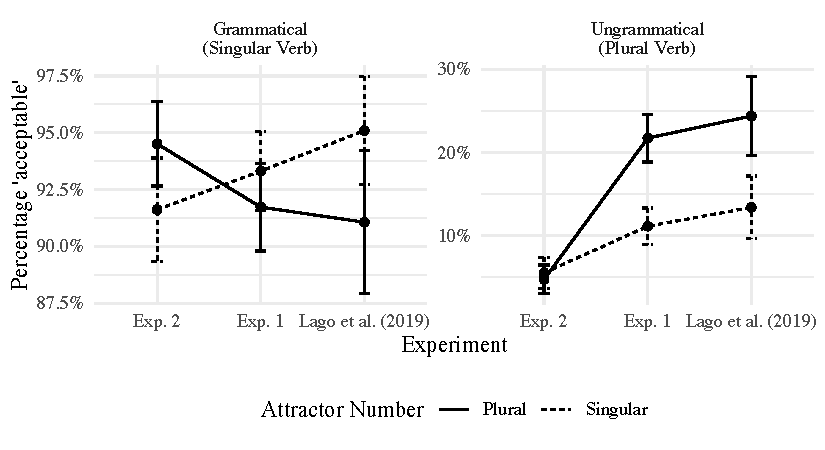
\includegraphics[width=\linewidth]{figure/exp2AvgResponse-1} 

}

\caption[The average percentage of acceptable responses according to the experimental conditions in Experiment 1, Experiment 2A, and Lago et al.'s (2019) study]{The average percentage of acceptable responses according to the experimental conditions in Experiment 1, Experiment 2A, and Lago et al.'s (2019) study}\label{fig:exp2AvgResponse}
\end{figure}

\end{knitrout}

We see that our results were comparable with previous findings of Turkish agreement attractions. Even though it is unusual that grammatical sentences with singular attractors (M = 0.92, SE = 0.01) compared to grammatical sentences with plural attractors (M = 0.95, SE = 0.01), given the standard errors, the difference between these two conditions do not seem to be significant. 

As for ungrammatical sentences, the mainstream agreement attraction effect, i.e., the effect of plural attractor on the acceptability of ungrammatical sentences was not present in Experiment 2. In Experiment 2, the ungrammatical sentences with plural attractors are rated as acceptable (M = 0.05, SE = 0.01) as their counterparts with singular attractors (M = 0.06, SE = 0.01). The lack of effect (0.01\%) compared to the magnitude of the effect in Experiment 1 (0.11\%) and \cites{LagoEtAl2019} study (0.11\%) indicates that the verbal plural morpheme does not trigger an illusionary agreement.

Figure \ref{fig:exp2RT} shows the average response times for correct responses by experimental conditions for our Experiment 2, Experiment 1, and \cites{LagoEtAl2019} study. We have used the same layout as the one we used in Figure \ref{fig:exp2AvgResponse}. However, this time we located Experiment 2 in the middle so that its relation to both our Experiment 1 and \cites{LagoEtAl2019} study can be observed easily.

\begin{knitrout}
\definecolor{shadecolor}{rgb}{0.969, 0.969, 0.969}\color{fgcolor}\begin{figure}[hbt!]

{\centering 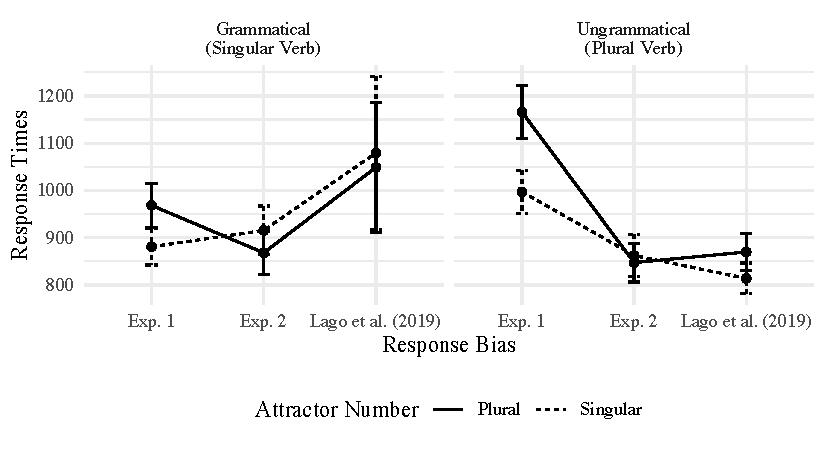
\includegraphics[width=\linewidth]{figure/exp2RT-1} 

}

\caption[The average response times according to the experimental conditions in Experiment 1, Experiment 2A, and Lago et al.'s (2019) study]{The average response times according to the experimental conditions in Experiment 1, Experiment 2A, and Lago et al.'s (2019) study}\label{fig:exp2RT}
\end{figure}

\end{knitrout}

Response Times in our Experiment 2 do neither align with our Experiment 1 nor with \cites{LagoEtAl2019} study fully. In the grammatical sentence, response times are comparable to our Experiment 1; however, the relation between the singular and plural attractor conditions is again reversed. Overall, participants took more time answering acceptability judgment questions to grammatical sentences with singular attractor (M = 915.28, SE = 26.32) compared to their plural attractor counterpart (M = 867.91, SE = 23.43). This difference does not seem to be substantial.

Within ungrammatical conditions, the picture is distinctively different from our findings in Experiment 1. There is no slowdown due to the presence of a plural attractor. Grammaticality judgment questions in both singular and plural attractor conditions were answered in a similar time (M = 862.31 and 847.23, SE = 22.82 and 20.87 for singular and plural attractor conditions, respectively). 

In Figure \ref{fig:exp2BayesPool}, we present the coefficient posterior summaries extracted from our Bayesian GLM fitted to the data from Experiment 1 and Experiment 2A. 


\begin{knitrout}
\definecolor{shadecolor}{rgb}{0.969, 0.969, 0.969}\color{fgcolor}\begin{figure}[hbt!]

{\centering 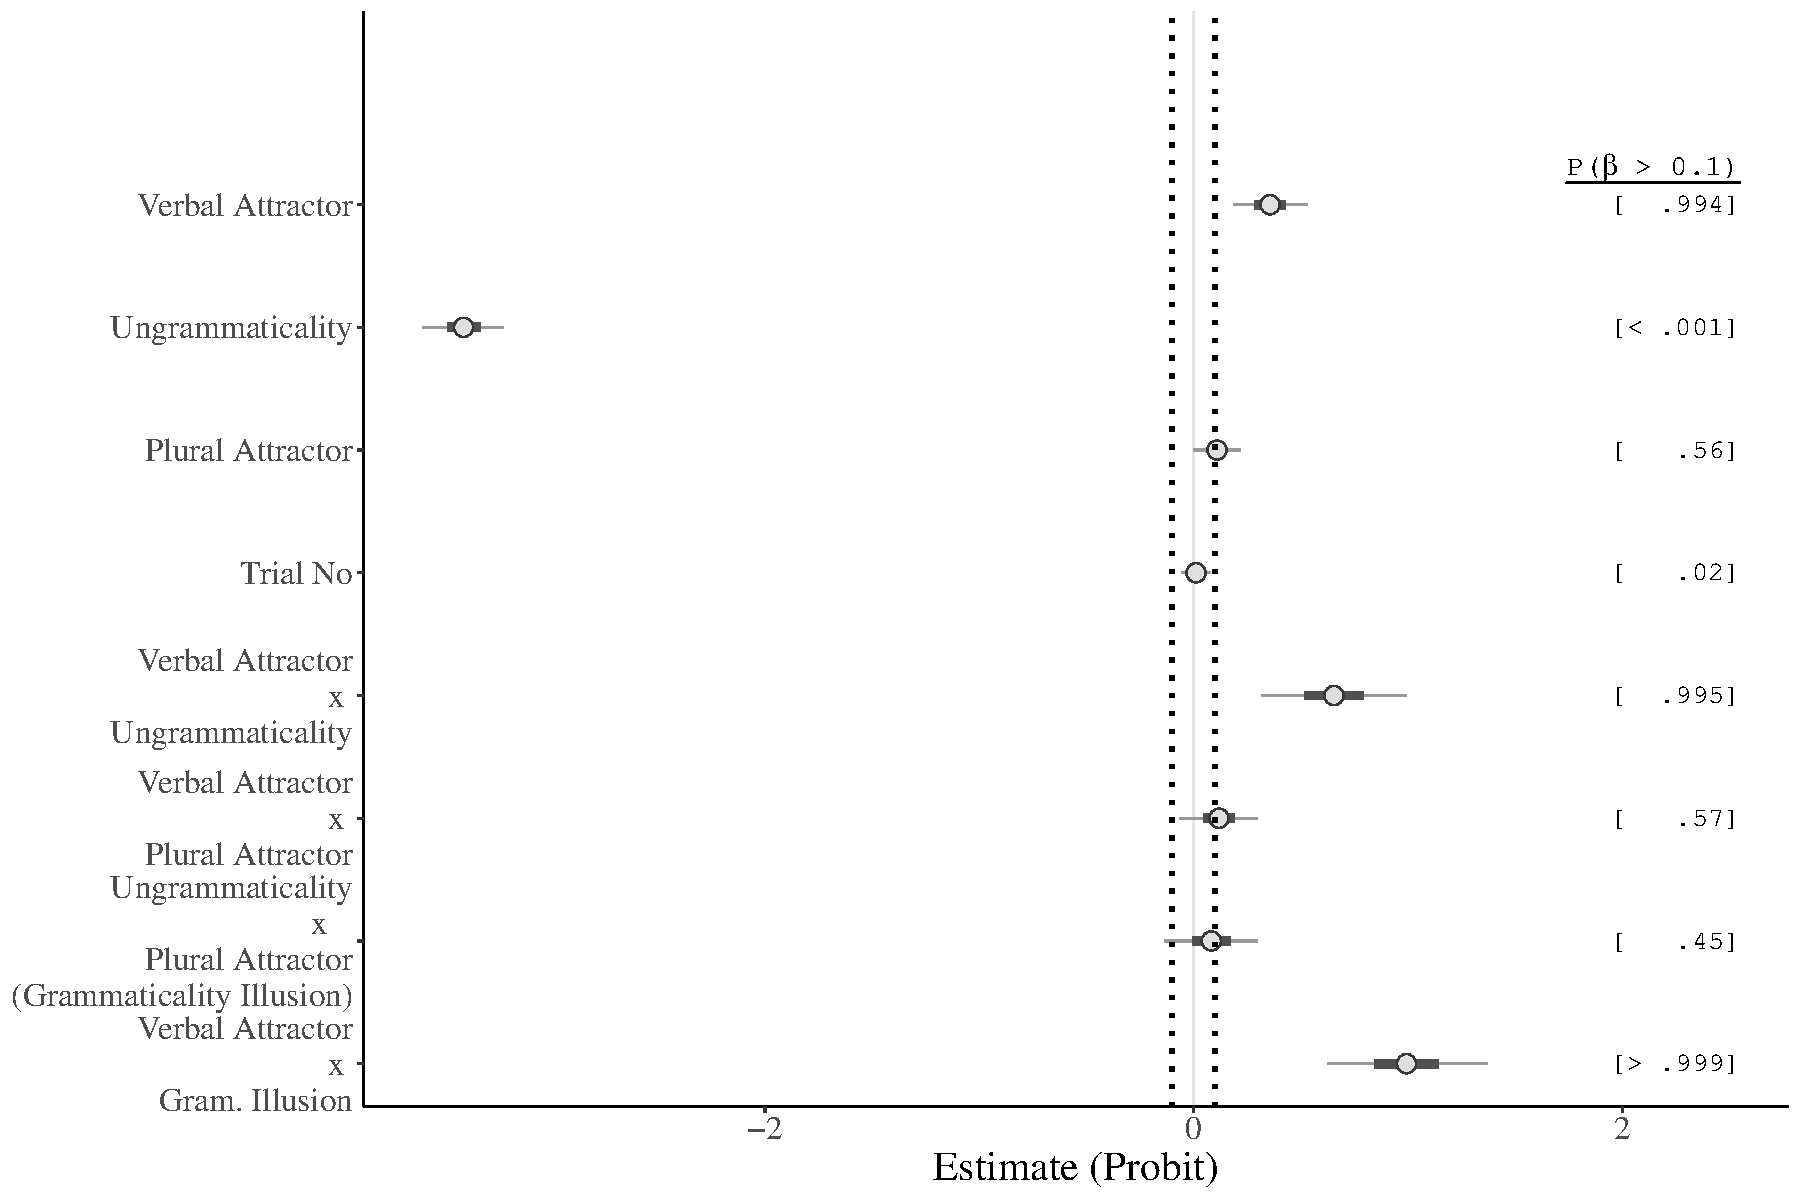
\includegraphics[width=\linewidth]{figure/exp2BayesPool-1} 

}

\caption[Estimates and 95\% credible intervals for the probit regression coefficients for the model of responses in Experiment 1 and Experiment 2A]{Estimates and 95\% credible intervals for the probit regression coefficients for the model of responses in Experiment 1 and Experiment 2A}\label{fig:exp2BayesPool}
\end{figure}

\end{knitrout}
The negative main effect of ungrammaticality ($\hat{\beta}=-3.41;$ $CI=[-3.64; -3.19];$ $P(\beta>0.1)< .001$) suggests that participants gave detected the ungrammaticality easily. The positive main effect of the genitive-marked nominal modifier ($\hat{\beta}=0.36;$ $CI=[0.15; 0.56];$ $P(\beta>0.1)  .994$) suggest that participants overall have more difficulty in correctly judging ungrammatical sentences in the presence of a nominal attractor compared to a verbal one. The positive interaction between the genitive-marked nominal attractor and the ungrammaticality ($\hat{\beta}=0.65;$ $CI=[0.25; 1.06];$ $P(\beta>0.1)  .995$) showed that participants made more errors in ungrammatical sentences when the nominal attractor is present instead of a verbal attractor independent of the presence of a plural attractor. More importantly, the positive three-way interaction ($\hat{\beta}=0.99;$ $CI=[0.55; 1.45];$ $P(\beta>0.1)> .999$) implies that the effect of nominal modifiers was even more amplified when they judge ungrammatical sentences with plural attractors compared to their counterparts with singular attractors. 

% font and resizing. May 1 11:51



Figure \ref{fig:exp2Bayesonly2} shows the estimates of our model fitted only to the data from Experiment 2. While Figure \ref{fig:exp2BayesPool} indicates the greater magnitude of agreement attraction effects with genitive attractors, it does not clearly show whether or not there exists a grammaticality illusion with verbal attractors. The negative interaction between grammaticality and plural attractor ($\hat{\beta}=-0.25;$ $CI=[-0.65; 0.17];$ $P(\beta>0.1)   .05$) shows that the presence of a plural marked verbal element in the vicinity of the head noun made participants give yes responses less often as opposed to having a singular marked verbal element. This interaction can also be interpreted as an amplified number of yes responses in grammatical sentences with plural attractors. 


\begin{knitrout}
\definecolor{shadecolor}{rgb}{0.969, 0.969, 0.969}\color{fgcolor}\begin{figure}[hbt!]

{\centering 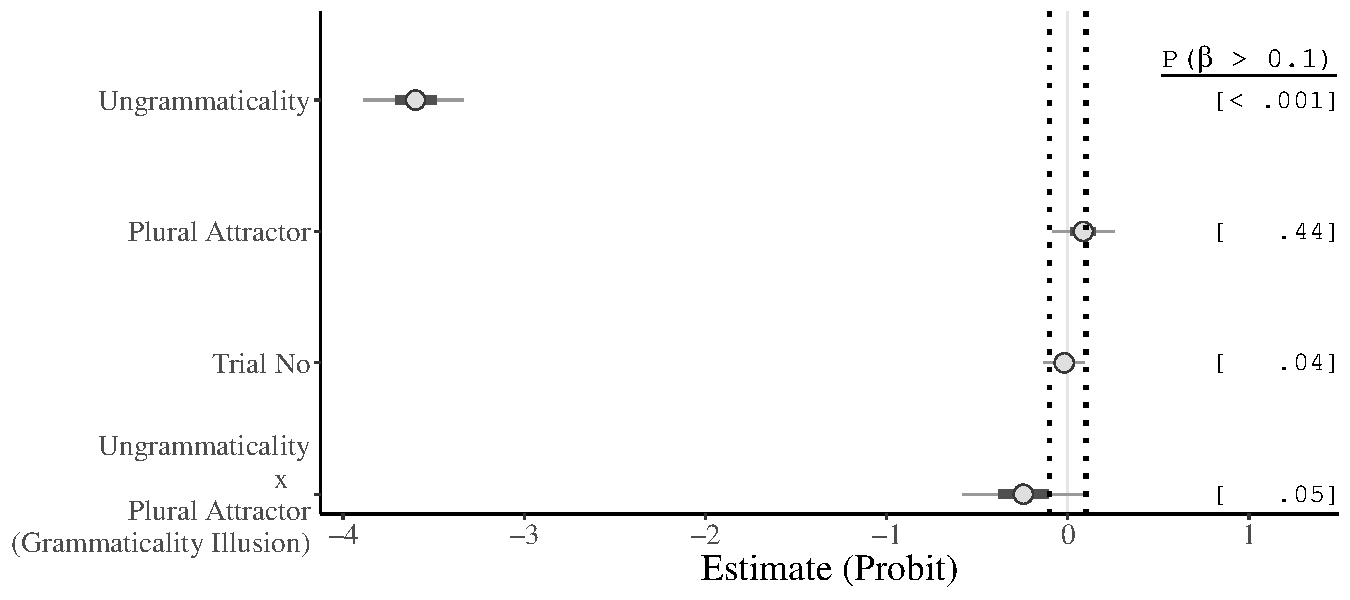
\includegraphics[width=\linewidth]{figure/exp2Bayesonly2-1} 

}

\caption[Estimates and 95\% credible intervals for the probit regression coefficients for the model of responses in Experiment 2 only]{Estimates and 95\% credible intervals for the probit regression coefficients for the model of responses in Experiment 2 only}\label{fig:exp2Bayesonly2}
\end{figure}

\end{knitrout}

\subsection{Discussion}


Experiment 2A examined an alternative hypothesis for Turkish agreement attraction facts. We hypothesized that participants might have formed a form-driven processing strategy and employed a shallow processing in the previous experiments. Assuming that most of the yes responses in ungrammatical conditions come from guesses, either completely random guesses or slightly informed ones, we argued that participants might solely rely on the foggy memory of a plural-marking in the sentence. On some occasions, where they misremembered the host of the plural-marking, they might erroneously judge sentences grammatical even though the head was singular. 

Results of our speeded acceptability judgment experiment showed that verbs of reduced object relative clauses were not appropriate attractors and there was no attraction effects with verbal attractors. However, number agreement attractions were observed in our previous experiment when the attractors were nominal. Even though the surface morphological form was identical for both verbal and nominal plural morphemes, the contributions of these two \emph{-lAr} morphemes to attraction effects differed. This finding contradicted our hypothesized form-driven processing strategy and supported an account of agreement attraction based on abstract linguistic features, rather than mere forms.

However, one possible explanation for Experiment 2 results is that participants never considered \emph{-lAr} morpheme to be hosted by a controller. They neither had any item that contained a plural head noun nor any experimental condition which would induce an erroneous agreement. Given that nominal attractors embedded more deeply in relative clauses than prepositional phrases cause less agreement attraction effects, a visible effect of an embedded verbal attractor in our experiment would be highly improbable. We believe that a limited number of grammatical filler items where the initial RC was marked with a plural agreement was not enough to lead participants to correlate the suffix \emph{-lAr} and the grammaticality potentially. 

Given these reasons, we pooled experimental conditions from Experiment 1 and 2A and conducted another study with eight conditions (Grammaticality x Attractor Number x Attractor Type). We already observed that in two different populations (\citeand{LagoEtAl2019} and Experiment 1), genitive-marked attractors cause agreement attraction and erroneous subject-verb agreement. In the light of previous findings that suggest participants misinterpret the sentence and compute the attractors as the head noun \citep{PatsonHusband2016}, we hypothesized that participants would misinterpret some of the ungrammatical sentences with genitive-marked attractors, and thus create form-based strategies more easily after seeing a certain number of ungrammatical conditions with plural-marked genitive modifiers. 

\section{Experiment 2B}

The aim of Experiment 2B is to again check for form-driven processing strategies but in a possibly more enabling experimental context. We believe that the presence of experimental conditions that possibly provide the necessary grammaticality illusion for participants to form a response strategy would give rise to mainstream attraction effects in relevant conditions with the embedded verbal attractor. Experiment 2B also provided a direct comparison in a single population between the nominal and embedded verbal attractor, which was also lacking in Experiment 2A.

\subsection{Participants}

Our participants (N = 95) were native Turkish speakers and Bo\u{g}azi\c{c}i University undergraduate students. In exchange for attending the experiment, they were given extra credit in one of the pre-determined Linguistics courses. The average age of participants was 21, ranging from 18 to 30. The principles of the Declaration of Helsinki and the regulations concerning research ethics at Bo\u{g}azi\c{c}i University were followed without any exception. Before the experiment, all participants were asked to provide informed consent. During the experiment, any information regarding their identities was not collected. 

\subsection{Materials}

In Experiment 2B, we have used 40 sets of experimental sentences where we manipulated the number of the attractor, the number agreement of the main verb, and the type of the attractor. We combined experimental items from Experiment 1 and 2A. We made sure that all eight conditions were minimally different. However, some of the items from Experiment 1 did not have the same head noun-matrix verb pair with those from Experiment 2A. For this reason, we modified some of the Experiment 1 sentences minimally. One item set is given below in (\ref{ex:exp2bitems}), where the subject phrase is marked with square brackets, and the dependency between the subject head and the matrix verb is signaled using bold-face.

\ea \label{ex:exp2bitems}
    \ea[*]{{Plural Verbal Attractor, Ungrammatical (Plural Verb)} \label{ex:exp2b-rcplpl}\\*
        \gll [{Tut-tuk-lar-{\i}} {a\c{s}\c{c}{\i}}] mutfak-ta sürekli z{\i}pla-d{\i}-lar.\\
        hire-\Nmlz{}-\Pl{}-\Poss{} cook kitchen-\Loc{} non-stop  jump-\Pst{}-\Pl{}\\
        \glt `The cook that they hired\textsubscript{\Pl{}} jumped\textsubscript{\Pl{}} in the kitchen non-stop.'}
    \ex[]{{Plural Verbal Attractor, Grammatical (Singular Verb)} \label{ex:exp2b-rcplsg} \\*
        \gll [{Tut-tuk-lar-{\i}} {a\c{s}\c{c}{\i}}] mutfak-ta sürekli z{\i}pla-d{\i}.\\
        hire-\Nmlz{}-\Pl{}-\Poss{} cook kitchen-\Loc{} non-stop  jump-\Pst{}\\
        \glt `The cook that they hired\textsubscript{\Pl{}} jumped\textsubscript{\Sg{}} in the kitchen non-stop.'}
    \ex[*]{{Singular Verbal Attractor, Ungrammatical (Plural Verb)} \label{ex:exp2b-rcsgpl}\\*
        \gll [{Tut-tu\u{g}-u} {a\c{s}\c{c}{\i}}] mutfak-ta sürekli z{\i}pla-d{\i}-lar.\\
        hire-\Nmlz{}-\Poss{} cook kitchen-\Loc{} non-stop  jump-\Pst{}-\Pl{}\\
        \glt `The cook that they hired\textsubscript{\Sg{}} jumped\textsubscript{\Pl{}} in the kitchen non-stop.'}
    \ex[]{{Singular Verbal Attractor Grammatical (Singular Verb)} \label{ex:exp2b-rcsgsg}\\*
        \gll [{Tut-tu\u{g}-u} {a\c{s}\c{c}{\i}}] mutfak-ta sürekli z{\i}pla-d{\i}.\\
        hire-\Nmlz{}-\Poss{} cook kitchen-\Loc{} non-stop  jump-\Pst{}\\
        \glt `The cook that they hired\textsubscript{\Sg{}} jumped\textsubscript{\Sg{}} in the kitchen non-stop.'}
    \ex[*]{{Plural Nominal Attractor, Ungrammatical (Plural Verb)} \label{ex:exp2b-genplpl}\\*
        \gll [{Y{\"o}netici-ler-in} {a\c{s}\c{c}{\i}-s{\i}}] mutfak-ta sürekli z{\i}pl-d{\i}-lar.\\
        manager-\Pl{}-\Gen{} cook-\Poss{} kitchen-\Loc{} non-stop  jump-\Pst{}-\Pl{}\\
        \glt `The millionaries' cook jumped\textsubscript{\Pl{}} in the kitchen non-stop.'}
    \ex[]{{Plural Nominal Attractor, Grammatical (Singular Verb)} \label{ex:exp2b-genplsg} \\*
        \gll [{Y{\"o}netici-ler-in} {a\c{s}\c{c}{\i}-s{\i}}] mutfak-ta sürekli z{\i}pl-d{\i}.\\
        manager-\Pl{}-\Gen{} cook-\Poss{} kitchen-\Loc{} non-stop  jump-\Pst{}\\
        \glt `The millionaries' cook jumped\textsubscript{\Sg{}} in the kitchen non-stop.'}
    \ex[*]{{Singular Nominal Attractor, Ungrammatical (Plural Verb)} \label{ex:exp2b-gensgpl}\\*
        \gll [{Y{\"o}netici-nin} {a\c{s}\c{c}{\i}-s{\i}}] mutfak-ta sürekli z{\i}pl-d{\i}-lar.\\
        manager-\Gen{} cook-\Poss{} kitchen-\Loc{} non-stop  jump-\Pst{}-\Pl{}\\
        \glt `The millionarie's cook jumped\textsubscript{\Pl{}} in the kitchen non-stop.'}
    \ex[]{{Singular Nominal Attractor, Grammatical (Singular Verb)} \label{ex:exp2b-gensgsg}\\*
        \gll [{Y{\"o}netici-nin} {a\c{s}\c{c}{\i}-s{\i}}] mutfak-ta sürekli z{\i}pl-d{\i}.\\
        manager-\Gen{} cook-\Poss{} kitchen-\Loc{} non-stop  jump-\Pst{}\\
        \glt `The millionarie's cook jumped\textsubscript{\Sg{}} in the kitchen non-stop.'}
    \z
\z

In addition to 40 experimental items, we also included 40 filler items, half of which are ungrammatical. We used the same filler items from Experiment 2A and did not modify any part of the fillers. All of our experimental and filler items can be found in Appendix \ref{ap:exp2bitems}.

\subsection{Procedure}

Experiment 2B was carried out in the same manner as Experiment 1 and 2A. 

\subsection{Analysis}

Since our main question was that participants used a response strategy based on form-matching and our Experiment 2B included both verbal and nominal attractors, we used only the experimental items from Experiment 2B. 

Similar to Experiment 1 and 2B, we removed all participants who did not exceed the threshold of 0.25 percentage points in yes responses between the grammatical condition and the ungrammatical condition with singular attractors. We also excluded trials where participants either gave too fast ($RT < $ 200 ms) or too slow ($RT > $ 4999 ms) responses. As a result, we excluded 2.34\% of trials from Experiment 2B.

We fitted two Bayesian GLMs to the yes responses from our Experiment 2B. While our first model included all experimental conditions, the second one only had verbal attractor conditions. We assumed that responses were distributed following a Bernoulli distribution with a probit link function. We used the R packages brms \citep{R-brms_a,R-brms_b} and rstan \citep{R-rstan} to fit Bayesian hierarchical models \citep[e.g.,][]{GelmanHill:2007, NicenboimVasishth:2016}. We analyzed only experimental sentences without including the missing data in the formula and used three categorical predictors and their interactions. We used (i) grammaticality of the sentence, (ii) attractor number, and (iii) the attractor type, as well as their interactions as predictors. We also included the log transformed trial number in our models ($l\_trial$). Moreover, we used by-participant and by-item intercepts and slopes for all predictors. All factors were sum-coded. We used 0.5 for the following levels: (i) ungrammaticality, (ii) plural attractor, and (iii) genitive-marked nominal modifier. We used the same priors as we used in previous Bayesian GLMs.

\subsection{Results}

In this section, we provide summaries of the coefficient posterior distributions. We ran 4 chains with 1000 warm-up iterations and 4000 sampling iterations for our models. Our results report the posterior probability of the effect of coefficient $\beta$ being outside of the ROPE region, either smaller than $-0.1$ (\emph{P}($\beta < -0.1$)) or bigger than $0.1$ (\emph{P}($\beta > 0.1$)). If a distribution is completely outside of this area, we can say that we have definitive evidence for an effect. If it covers the practical equivalence area, we can say that according to our data, there seems to be no evidence for an effect. On occasions in which only a part of the distribution resides in the area, we explicitly quantify our degree of belief towards an effect.

Both grammatical and ungrammatical fillers' accuracy were high (M = 0.95 and 0.94, SE = 0.01 and 0.01 for grammatical and ungrammatical fillers). We believe that our filler items served their purpose, and participants paid attention to the experiment. 

Figure \ref{fig:exp2bAvgResponse} shows the average proportions of acceptable responses for each experimental condition in Experiment 2B. We divided the results into two facets: grammatical and ungrammatical sentences. We have the attractor type (Genitive modifiers vs. Relative Clause modifiers as attractors) on the x-axis. Finally, the attractor number is represented with the line type. 

\begin{knitrout}
\definecolor{shadecolor}{rgb}{0.969, 0.969, 0.969}\color{fgcolor}\begin{figure}[hbt!]

{\centering 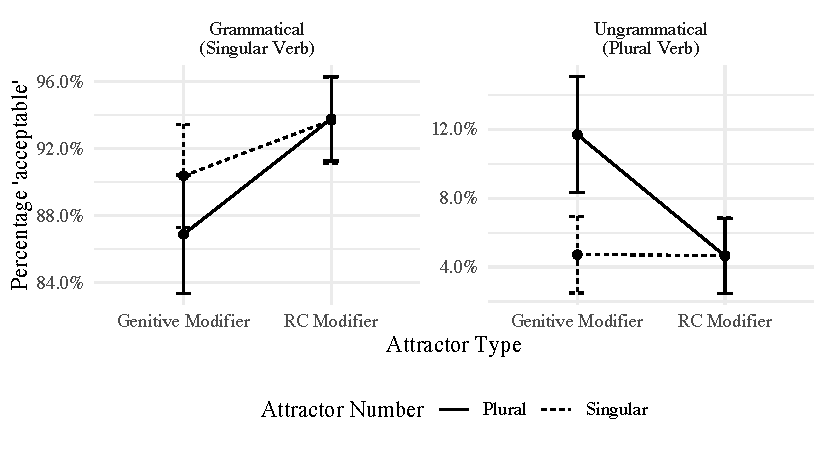
\includegraphics[width=\linewidth]{figure/exp2bAvgResponse-1} 

}

\caption[The average percentage of acceptable responses according to the experimental conditions in Experiment 2B]{The average percentage of acceptable responses according to the experimental conditions in Experiment 2B}\label{fig:exp2bAvgResponse}
\end{figure}

\end{knitrout}


In grammatical sentences, the overall acceptability was lower in genitive modifier conditions (ME = 0.87 and 0.9, SE = 0.02 and 0.02, for singular and plural attractors, respectively) compared to RC modifier conditions (ME = 0.94 and 0.94, SE = 0.01 and 0.01, for singular and plural attractors, respectively). 

In ungrammatical sentences, the plurality of the attractor did not change the overall attractor within RC modifier conditions (ME = 0.05 and 0.05, SE = 0.01 and 0.01, for singular and plural attractors, respectively). On the other hand, the attractor number mattered when the modifier was  a genitive-marked nominal. Participants accepted ungrammatical sentences with a plural genitive-marked nominal attractor (ME = 0.12, SE = 0.02) more often compared to the ones with a singular attractor (ME = 0.05, SE = 0.01). Even though this effect size (0.07) diminished compared to our previous agreement attraction findings (0.11), they were still comparable. This decrease in acceptability can be seen in Figure \ref{fig:exp2B1AvgResponse}. The layout in Figure \ref{fig:exp2B1AvgResponse} is the same as the previous figures. Differently from the rest, the x-axis represents the attractor type and the experiment.  

\begin{knitrout}
\definecolor{shadecolor}{rgb}{0.969, 0.969, 0.969}\color{fgcolor}\begin{figure}[hbt!]

{\centering 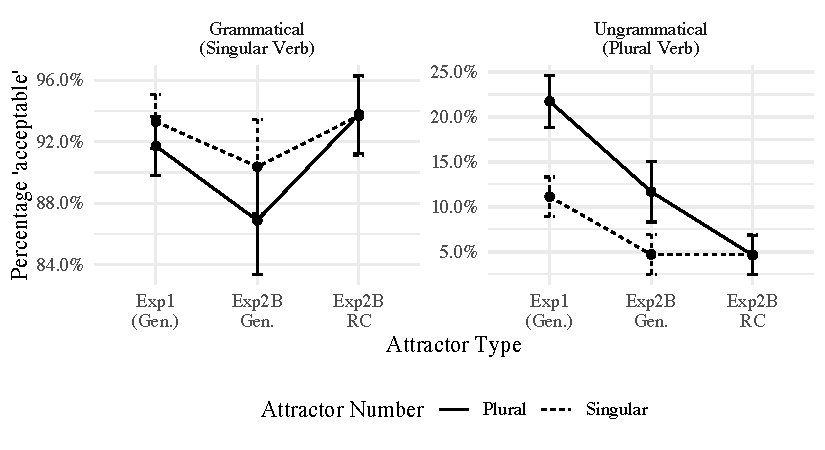
\includegraphics[width=\linewidth]{figure/exp2B1AvgResponse-1} 

}

\caption[The average percentage of acceptable responses according to the experimental conditions in Experiment 1 and Experiment 2B]{The average percentage of acceptable responses according to the experimental conditions in Experiment 1 and Experiment 2B}\label{fig:exp2B1AvgResponse}
\end{figure}

\end{knitrout}

Figure \ref{fig:exp2bRT} shows average response times for correct responses in Experiment 2B. We have used the same layout as in Figure \ref{fig:exp2bAvgResponse}.

\begin{knitrout}
\definecolor{shadecolor}{rgb}{0.969, 0.969, 0.969}\color{fgcolor}\begin{figure}[hbt!]

{\centering 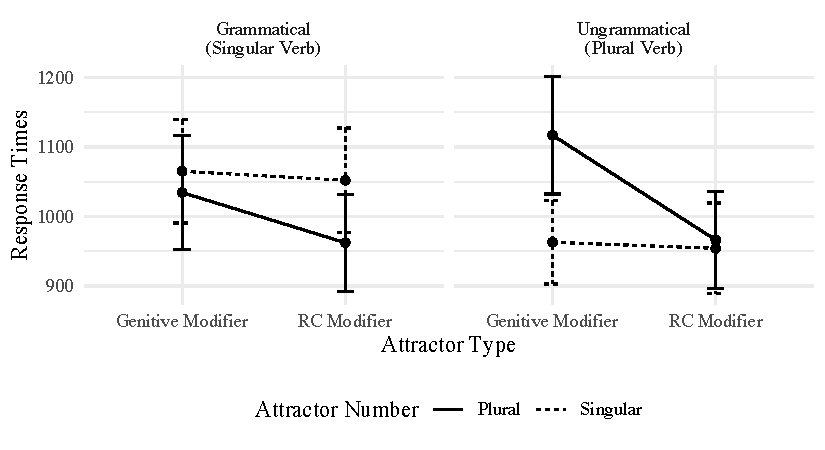
\includegraphics[width=\linewidth]{figure/exp2bRT-1} 

}

\caption[The average response times according to the experimental conditions in Experiment 2B]{The average response times according to the experimental conditions in Experiment 2B}\label{fig:exp2bRT}
\end{figure}

\end{knitrout}

Participants in our Experiment 2B responded faster to grammatical sentences with plural-marked attractors (M = 1034.45 and 962.22, SE = 41.88 and 35.55 for genitive and RC modifiers, respectively) compared to the ones with singular ones (M = 1065.04 and 1051.99, SE = 37.92 and 38.48 for genitive and RC modifiers, respectively). 

As for ungrammatical conditions, participants gave correct responses slower with plural genitive modifier (M = 1116.92, SE = 43.09) than the singular genitive modifier (M = 962.85, SE = 30.56). However, this difference in RT was not present in RC modifier conditions (M = 954.04 and 966.21, SE = 33.28 and 35.69 for singular and plural RCs, respectively). 


In Figure \ref{fig:exp2bBayes}, we present the coefficient posterior summaries from our Bayesian GLM fitted to experimental sentences from Experiment 2B. 


\begin{figure}[hbt!]

{\centering 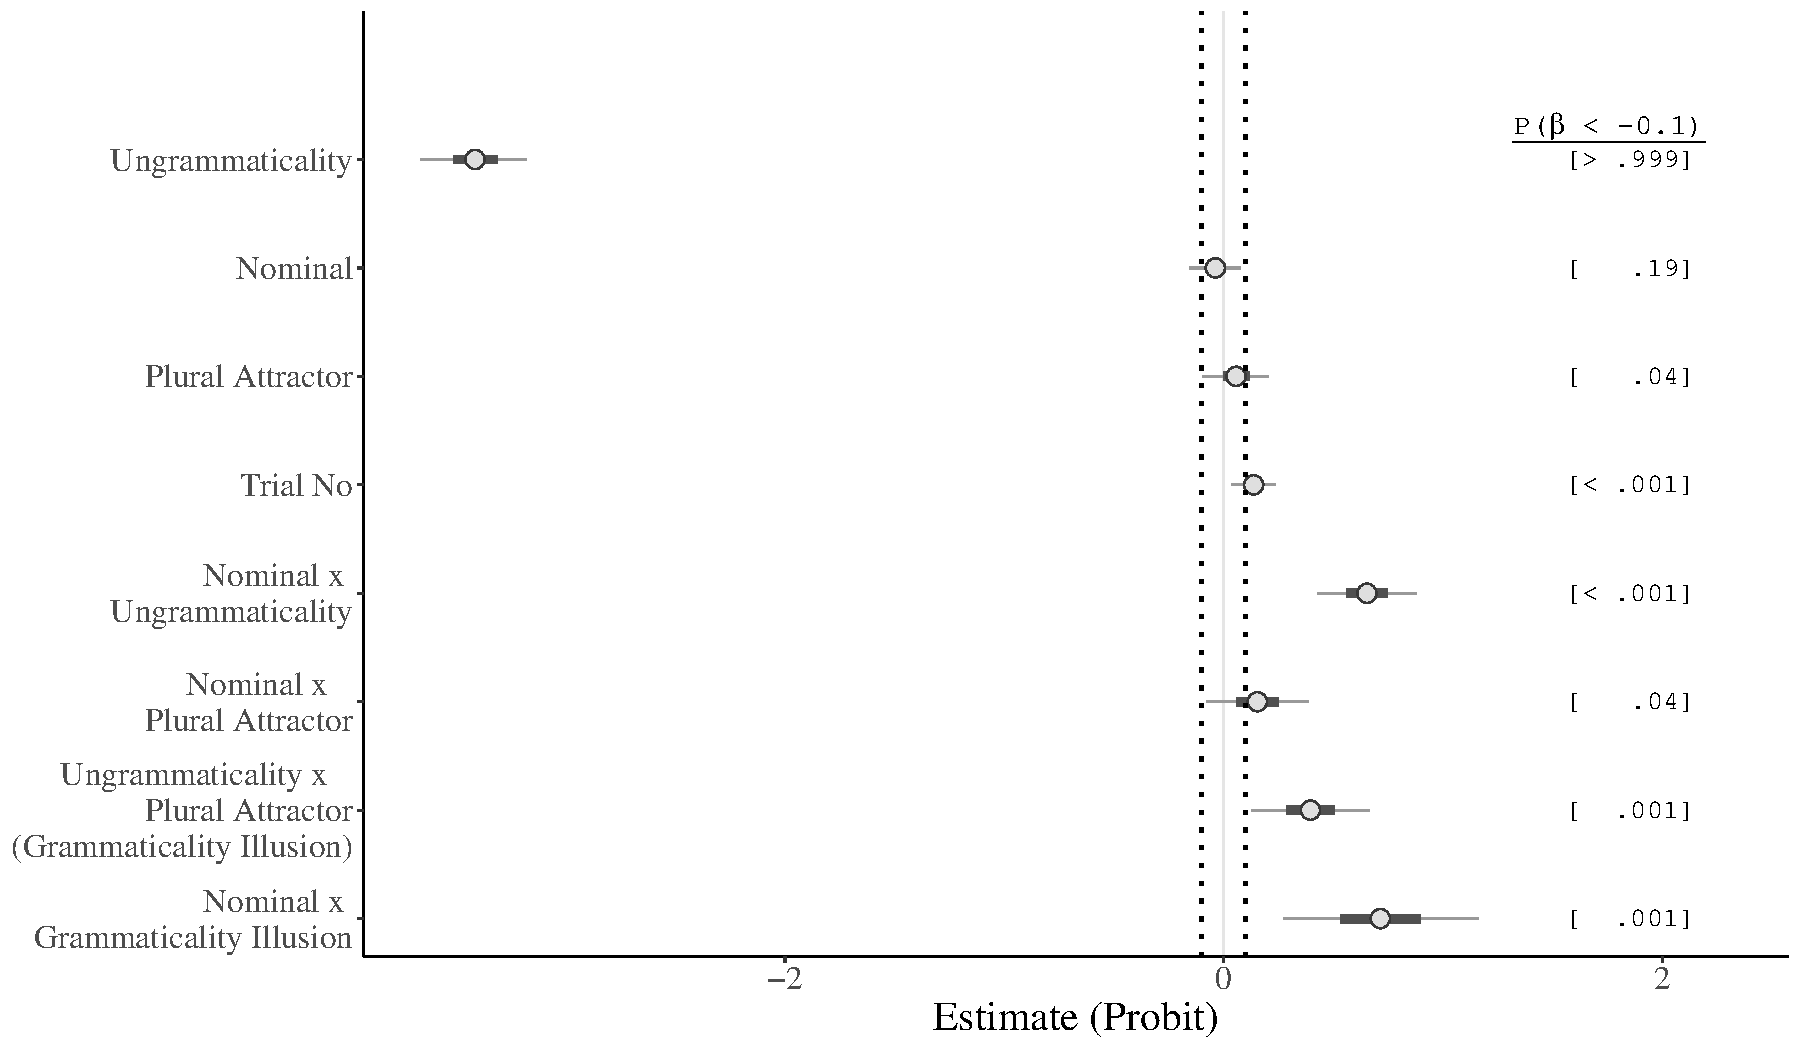
\includegraphics[width=\linewidth]{figure/exp2bBayes-1} 

}

\caption[Estimates and 95\% credible intervals for the probit regression coefficients for the model of responses in Experiment 2B]{Estimates and 95\% credible intervals for the probit regression coefficients for the model of responses in Experiment 2B}\label{fig:exp2bBayes}
\end{figure}

The negative main effect of ungrammaticality ($\hat{\beta}=-3.41;$ $CI=[-3.72; -3.14];$ $P(\beta< -0.1)> .999$) was also present in this Bayesian GLM as well. Participants were able to differentiate between the grammatical and ungrammatical items within experimental items. Our posterior summaries showed a positive effect of the trial number ($\hat{\beta}=0.14;$ $CI=[0.02; 0.26];$ $P(\beta< -0.1)< .001$), meaning that as participants see more experimental items, they gave more yes responses, on average. This effect suggested that participants might change how they answered questions as they proceeded in the experiment. The positive three-way interaction between the type of the attractor, ungrammaticality, and the plurality of the attractor ($\hat{\beta}=0.71;$ $CI=[0.18; 1.26];$ $P(\beta< -0.1)=   .001$) implied that the mainstream attraction effect (Ungrammaticality * Plural Attractor interaction) was amplified when the attractor is a genitive-marked nominal modifier.


However, this three-way interaction did not prove that people exhibited agreement attraction effects with verbal modifiers. Figure \ref{fig:exp2bRCBayes} shows coefficient posteriors for our second Bayesian GLM, fitted only the experimental items with verbal modifiers. We see that there was an evidence for neither an effect of plural attractor ($\hat{\beta}=-0.07;$ $CI=[-0.41; 0.25];$ $P(\beta< -0.1)=    .42$) nor an interaction between the ungrammaticality and the plural attractor ($\hat{\beta}=0.25;$ $CI=[-0.29; 0.82];$ $P(\beta< -0.1)=    .10$). 

\begin{knitrout}
\definecolor{shadecolor}{rgb}{0.969, 0.969, 0.969}\color{fgcolor}\begin{figure}[hbt!]

{\centering 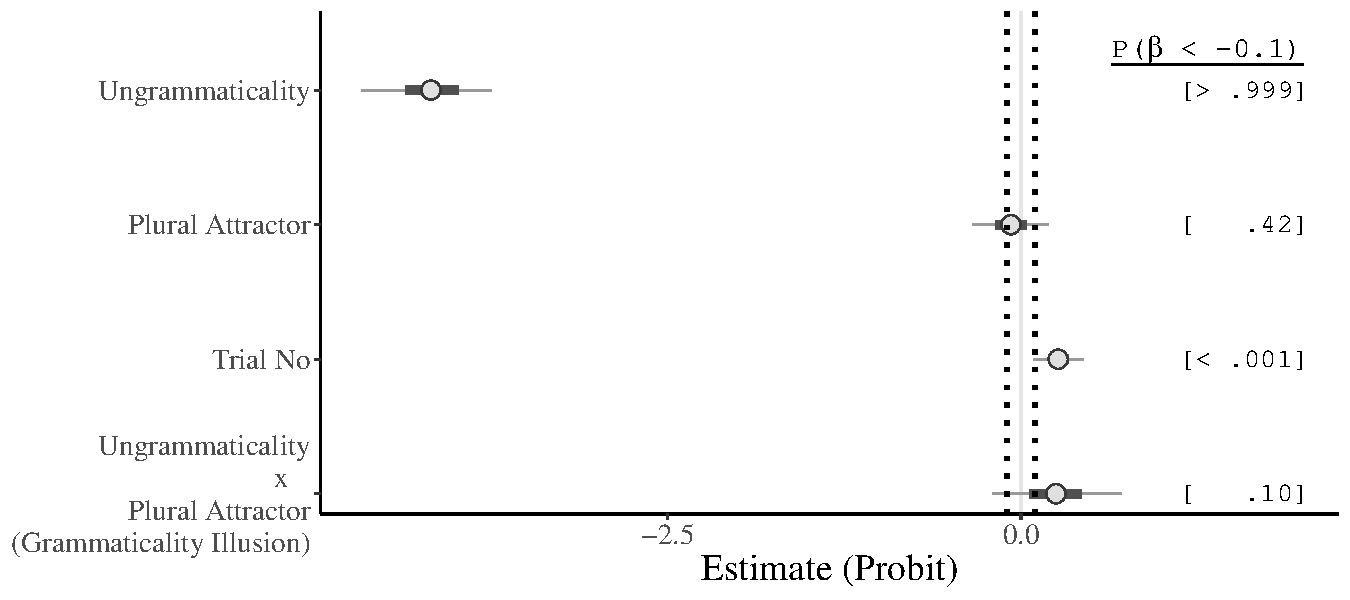
\includegraphics[width=\linewidth]{figure/exp2bRCBayes-1} 

}

\caption[Estimates and 95\% credible intervals for the probit regression coefficients for the model of responses to RC conditions in Experiment 2B]{Estimates and 95\% credible intervals for the probit regression coefficients for the model of responses to RC conditions in Experiment 2B}\label{fig:exp2bRCBayes}
\end{figure}

\end{knitrout}

\subsection{Discussion}

In Experiment 2B, we re-examined our hypothesis, according to which participants may form a response strategy using a form-matching mechanism. Even though our previous study, Experiment 2A, showed no evidence for such a strategy, we wanted to verify these findings with a new experiment. One possibility is that since there was no agreement controller with plural marking in Experiment 2A, participants might have never considered the form-matching response strategy. We included additional conditions, with genitive-marked modifiers which might lead participants to erroneously deem plural attractor DPs as agreement controllers and consider that the suffix \emph{-lAr} can be hosted by the head noun as well.

Our results showed that participants made significantly fewer errors in ungrammatical sentences when the attractor was verbal compared to nominal attractors. We successfully replicated our findings in Experiment 2A. Even though we included new genitive-modifier conditions to trigger agreement attraction effects in verbal attractors, it did not affect our participants. Together with Experiment 2A, Experiment 2B findings verified that our hypothesized decision-making process would not explain the patterns in Turkish agreement attraction effects.  

% The relationship with trial no and agreement attraction maybe?

\section{Discussion}

This chapter investigated another alternative hypothesis that might explain Turkish agreement attraction facts. We hypothesized that when participants did not have sufficient information to judge sentences' acceptability, they might use other heuristics such as form-matching strategies. Given that participants do not always process the sentences fully and utilize shallow processing methods, agreement attraction effects might be residual of a guessing mechanism. While some yes responses come from truly random guesses due to not having any memory regarding the subject-verb dependency, some yes responses come from educated guesses where participants have some sort of information that they can use. In our case, the additional information was the recollecting the presence of the plural suffix \emph{-lAr}. We argued that when people read sentences, sometimes they will remember and analyze the whole sentence. On the other hand, they will sometimes have a recollection uncertainty and misremember the host which the suffix \emph{-lAr} is concatenated. On those occasions, they will use a response strategy where they try to match two homophonous suffixes to answer grammaticality judgment questions.

Our MPT model differentiates these informed guesses from random guessing by either adjusting the relative probabilities of guessing yes ($g$) and no ($1-g$) or providing an additional probabilistic state before guessing. The product of this new state's probability and the standard guessing yes probability will be our way of formalizing the informed guesses ($(1-r){\ }\times{\ }g$). We conducted a speeded acceptability judgment experiment to test our hypothesis that participants with relocation uncertainty may utilize form-related response strategies. We investigated whether or not agreement-wise unrelated morphemes can trigger agreement attraction effects. We argued that if people utilize this form-driven processing strategy, they may give more yes responses even when there are verbal plural attractors in the vicinity compared to no plural attractor in the vicinity. We were able to test this hypothesis using Turkish since both verbal and nominal plurality is shown via the same morpheme: \emph{-lAr}.

Our results from two experiments, where we used verbs of a reduced object relative clauses as an attractor, showed that the usual effect of the plural attractor in ungrammatical sentences did not arise when the attractor is a verbal element. We expected that if participants were using our hypothesized response strategy, they would accept ungrammatical sentences with a plural attractor independent of the type of the attractor. However, this was not the case. Our findings contradicted our hypothesis and implied that participants used abstract linguistic features rather than form-related cues. Given our results, it was evident that the type of the attractor and the nature of the plural morpheme mattered in processing subject-verb dependencies. 

Moreover, our results from Experiment 2B showed a slight decrease in the overall percentage of yes responses in ungrammatical sentences with a nominal attractor. A possible explanation for this decrease might be the presence of verbal attractors. Their presence might have affected participants' sensitivity and made them more conservative in giving yes responses. The decrease in grammatical sentences supports this hypothesis. However, our experimental design and results are not equipped to answer this question. Thus, all we can say is that we have minimal evidence for such a speculation.

Lastly, we must note that our experiment designs were not without problems. Even though we compare the contributions of verbal and nominal attractors, they are not on par syntactically. We provide syntactic structures in (\ref{syntax:genposs}) and (\ref{syntax:orc}). To visualize syntactic differences between the structures, we mark the nodes between the root node and the node attractor is immediately dominated. The verbal attractor is embedded in a relative clause, consisting of DP, \emph{n}P, TP, \emph{v}P, and VP \citep{Aygen2002}. This relative clause is the modifier of the DP. On the other hand, the genitive-marked nominal modifier is the specifier of the determiner phrase, and it is immediately dominated by the root node \cite{OzturkTaylan2016}. It is clear that the syntactic distance between the root and the attractor nodes is more considerable with the verbal attractor.


\ea 
\ea \label{syntax:orc} {Object Relative Clause}\\*
\scalebox{1}{\begin{forest}
%fned
    [DP
        [DP
                [\emph{n}P
                    [TP
                        [DP\\\emph{pro}\textsubscript{j}]
                        [TP
                            [\emph{v}P
                                [DP\\\emph{t}\textsubscript{j}]
                                [\emph{v}P
                                    [VP
                                        [DP\\\emph{t}\textsubscript{i}]
                                    [V\\tuttuklar{\i}]
                                ]
                                [\emph{v}]
                            ]
                        ]
                        [T]
                    ]
                ]
                [\emph{n}]
            ]
            [D]
        ]
        [DP
            [NP [N\\a\c{s}\c{c}{\i}\textsubscript{i}] ]
            [D]
        ]
    ]
    \path[fill=black] (.parent anchor) circle[radius=2pt];
    \path[fill=black] (!1.child anchor) circle[radius=2pt];
    \path[fill=black] (!11.child anchor) circle[radius=2pt];
    \path[fill=black] (!111.child anchor) circle[radius=2pt];
    \path[fill=black] (!1112.child anchor) circle[radius=2pt];
    \path[fill=black] (!11121.child anchor) circle[radius=2pt];
    \path[fill=black] (!111212.child anchor) circle[radius=2pt];
    \path[fill=black] (!1112121.child anchor) circle[radius=2pt];
    \path[fill=black] (!11121212.child anchor) circle[radius=2pt];
\end{forest}}\vspace{2em}

\ex \label{syntax:genposs} {Genitive-Possessive DP}\\*
\scalebox{0.9}{\begin{forest}
    %fned
        [DP
            [DP\textsubscript{i}
                [PlP
                    [NP [NP\\Y\"onetici] ]
                    [Pl\\-ler]
                ]
                [D\\-in]
            ]
            [DP
                [\emph{n}P
                    [DP\\\emph{t}\textsubscript{i}]
                    [\emph{n}P
                        [NP [N\\a\c{s}\c{c}{\i}]]
                        [\emph{n}\\-s{\i}]
                    ]
                ]
                [D]
            ]
        ]
        \path[fill=black] (.parent anchor) circle[radius=2pt];
        \path[fill=black] (!1.child anchor) circle[radius=2pt];
        \path[fill=black] (!11.child anchor) circle[radius=2pt];
        \path[fill=black] (!112.child anchor) circle[radius=2pt];
    \end{forest}}
\z
\z


One reason for the failure of triggering grammaticality illusion in Experiment 2B might be the syntactic distance discrepancy between the conditions. Previous studies have shown that syntactic distance between the head and the modifier affects the magnitude of the attraction. The more embedded attractors resulted in smaller effects of plural attractors in ungrammatical sentences. A better experimental design for comparing between a nominal and a verbal attractor would include objects/subjects of an embedded RC instead of a genitive-marked nominal modifier that is not embedded under CP and TP. Even though there are multiple studies that shown clause-external attractors or attractors in embedded sentences induce agreement attraction, Turkish has not been tested yet.
